\documentclass[
    UTF8
]{report}

% page size setting
\usepackage{geometry}

% layout
\usepackage{multicol}

% using [H] to ban the float of algorithm, figure and so on.
\usepackage{float}

% insert pdf page
\usepackage{pdfpages}

% color
\usepackage{xcolor}

% figure
\usepackage{graphicx}
\usepackage[]{subfig}

% table
\usepackage{multirow}
\usepackage{array}

% math
\usepackage{amsmath}
\usepackage{amssymb}
% some custom math symbols
\newcommand{\vect}[1]{\boldsymbol{#1}} % vector
\newcommand{\mat}[1]{\mathbf{#1}}      % matrix
\newcommand{\tensor}[1]{\mathsf{#1}}   % tensor
\newcommand{\set}[1]{\mathbb{#1}}      % set
\newcommand{\T}{\mathrm{T}}        % transposition
\everymath{\displaystyle}              % block style for inline math


% code
%% float of algorithm
\usepackage{algorithm}
%% body of algorithm
\usepackage{algorithmic}
%% custom setting for algorithmic
\renewcommand{\algorithmicrequire}{\textbf{Input:}}
\renewcommand{\algorithmicensure}{\textbf{Output:}}
%% highlight
\usepackage{minted}

\usepackage{multicol}

% reference
\usepackage[]{hyperref}
\hypersetup{
    colorlinks=true,
}

% URL
\usepackage{url}
\usepackage[style=ieee]{biblatex}
\addbibresource{ref.bib}

\usepackage{lipsum}
% Text decoration
\usepackage{soul}
\usepackage{ulem}
% Indent first line automatically
\usepackage{indentfirst}
\newcommand{\algorithmautorefname}{Algorithm}
\newcommand{\subfigureautorefname}{Figure}
\renewcommand{\subsectionautorefname}{Subsection}
\renewcommand{\sectionautorefname}{Section}

\title{\LaTeX Template for English Report}
\author{Your name}
\date{\today}

\begin{document}

\pagestyle{plain}
\setcounter{page}{1}
\pagenumbering{Roman}
\maketitle
{
    \hypersetup{linkcolor=black}
    \tableofcontents
    \newpage
}
\setcounter{page}{1}
\pagenumbering{arabic}
\pagestyle{headings}

\chapter{\LaTeX}
\label{chapter:example}

\section{Text}

\begin{enumerate}
    \item normal
    \item \textbf{bold}
    \item \textit{italic}
    \item \sout{delete line}
    \item \xout{italic delete line}
    \item \uwave{wave}
    \item \underline{underline}
    \item \uline{underline}
    \item \uuline{double underline}
    \item \dashuline{dash underline}
    \item \dotuline{dot underline}
    \item \colorbox{yellow}{highlight}
\end{enumerate}

\section{Figure}

\subsection{One Figure}

\begin{figure}[H]
    \centering
    
\includegraphics[width=0.7\textwidth]{./img/logo.png}
    \caption{Logo of SCUT}
    \label{fig:logo}
\end{figure}

\subsection{Subfigure}

\begin{figure}[H]
    \centering
    \subfloat[subfig 1\label{fig:subfig-1}]{
        
\includegraphics[width=0.12\textwidth]{./img/logo-short.png}
    }
    \hspace{1em}
    \subfloat[subfig 2\label{fig:subfig-2}]{
        
\includegraphics[width=0.5\textwidth]{./img/logo.png}
    }
    ~\\
    \subfloat[subfig 3\label{fig:subfig-3}]{
        
\includegraphics[width=0.5\textwidth]{./img/logo.png}
    }
    \hspace{1em}
    \subfloat[subfig 4\label{fig:subfig-4}]{
        
\includegraphics[width=0.12\textwidth]{./img/logo-short.png}
    }
    \caption{subfigures}
    \label{fig:subfig}
\end{figure}

\section{Table}
\begin{table}[H]
    \centering
    \caption{Paramter Value}
    \label{tb:paramter}
    \begin{tabular}{c|c}
    \hline
    Parameter & Value \\ \hline
    $\alpha$  & 1     \\ \hline
    $\beta$   & 1     \\ \hline
\end{tabular}
\end{table}
\begin{table}[H]
    \centering
    \caption{Paramter Value}
    \label{tb:figure}
    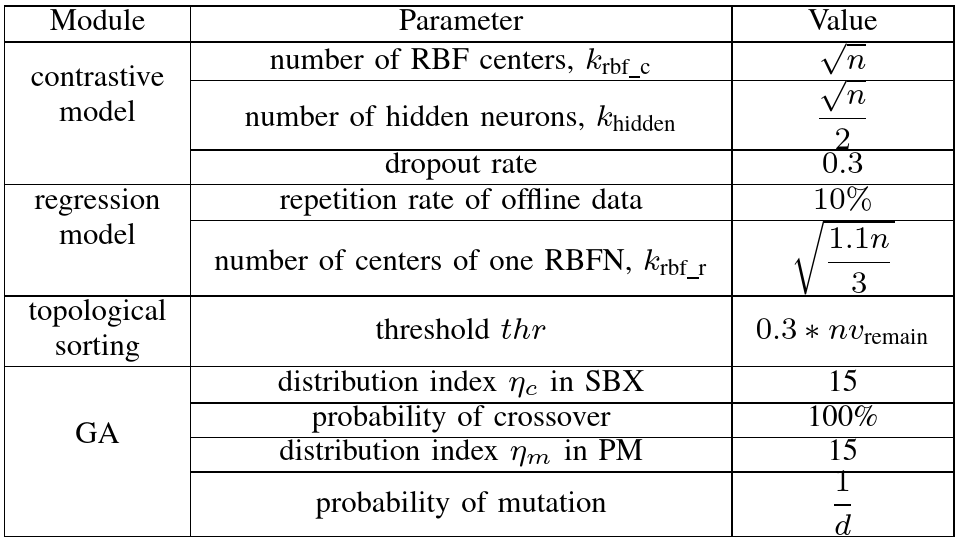
\includegraphics[width=0.65\textwidth]{./table/figure.png}
\end{table}
You cant take a screenshot, and throw the picture into the table environment, such as the table aboved.

\section{Pseudo-code}
\begin{center}
    \begin{minipage}{0.55\textwidth}
        \begin{algorithm}[H]
            \centering
            \caption{KahnAlgorithm}
            \label{algo:kaha}
            \begin{algorithmic}[1]
    \REQUIRE Graph $G(\mathbb{V}, \mathbb{E})$
    \ENSURE Sequence $L$
    \STATE $L \leftarrow$ an empty sequence
    \STATE $Q \leftarrow$ the vertices whose indegree is zero
    \WHILE{$Q$ is not empty}
        \STATE $u \leftarrow$ remove the top node of $Q$
        \STATE add $u$ to $L$
        \FOR{each node $v$ with an edge $e$ from $u$ to $v$}
            \STATE remove edge $e$ from graph $G$
            \IF{indegree of $v$ is $0$}
                \STATE push $v$ to $Q$
            \ENDIF
        \ENDFOR
    \ENDWHILE
    \RETURN $L$
\end{algorithmic}
        \end{algorithm}
    \end{minipage}
\end{center}

\begin{center}
    \begin{minipage}{0.55\textwidth}
        \begin{algorithm}[H]
            \scriptsize
            \caption{Framework}
            \label{aglo:figure}
            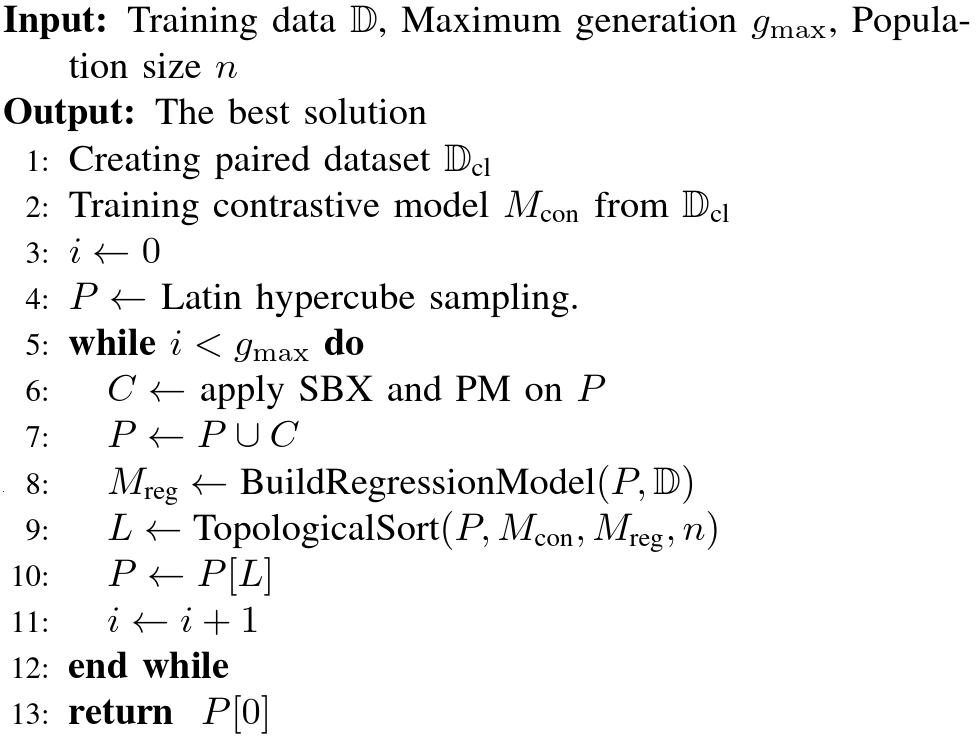
\includegraphics[width=\textwidth]{./algo/figure.png}
        \end{algorithm}
    \end{minipage}
\end{center}
You take a screenshot, and throw the picture into the algorithm environment, such as the algorithm aboved.

\section{Highlight}

\inputminted[linenos]{cpp}{./code/quicksort.cpp}

\section{Multiple Columns}
\begin{multicols}{2}
    \lipsum[1-3]
\end{multicols}

\section{Math}

Interline Formula:
\begin{equation}
    \label{eq:example}
    a_n = a_{n-1} + 1
\end{equation}

Inline Formula:
This is a simple arithmetic progression formula $a_n = a_{n-1} + 1$.

\section{Ref}
\begin{itemize}
    \item figure: \autoref{fig:logo}
    \item subfigure: \autoref{fig:subfig-1}
    \item table: \autoref{tb:paramter}
    \item pseudo-code: \autoref{algo:kaha}
    \item equation: \autoref{eq:example}
    \item chapter: \autoref{chapter:example}
    \item paper: \cite{he2016deep}
    \item url 1: \href{https://baidu.com}{baidu}
    \item url 2: \url{https://baidu.com}
\end{itemize}


\printbibliography[title={Reference}]

\end{document}